\chapter{Telemanipulátor geometriája}
\label{sec:geometria}

A szakdolgozatomban elkészített telemanipulátor koncepcionális újragondolását és a kompenzációs elvárásokat az előző fejezetben bemutattam. Az elvárás rendszer figyelembevételével megterveztem a telemanipulátor geometriai vázát.

A diploma dolgozatomban bemutatásra kerülő telemanipulátor geometriájának megtervezése több féléves munka után nyerte el végső formáját. A tervezési lépéseket a kompenzáció miatt szükséges elvi felépítéstől indulva minden lényegesebb elemen áthaladva mutatom be. Végül a kinematikai felépítését és a TCP pont számításához szükséges elemzéssel zárnám a fejezetet.

%----------------------------------------------------------------------------
\section{Geometria kialakítása}
%----------------------------------------------------------------------------

A kompenzációnál megemlített paralelogramma elrendezés használata rendkívül hasznos megoldásnak bizonyult és az egyik legnagyobb fejlesztésnek tartam a szakdolgozatban dokumentált munkámhoz képest. A paralelogramma elrendezés
miatt a kábel csatornák száma az ötödik csuklóig meg kétszereződött, mivel karonként kétszer annyi elem áll rendelkezésre. Ezen túl a rendszer stabilitását is növelte az által, hogy nehezebb csavaró vagy nyíró jellegű igénybe vétellel a csuklókat terhelni. Előnyként mutatkozott ez az elrendezés akkor is amikor a számításokat végeztem, mivel a paralelogramma elrendezés azt eredményezi, hogy a minden oldala a kinematikának párhuzamos marad a vele szemköztivel. Az ötödik csuklóig így csak szinusz koszinusz számításokat és egy darab transzformációt kellett elvégeznem. Az általam elképzelt telemanipulátor kinematikai elrendezése a következő lett. A rendszer egészében $6[db]$ csuklóban mérendő szögváltozó elmozdulása alapján tudja meghatározni a TCP pontot. A elvárások alapján két darab paralelogramma kinematikai összeállítást használok és ezt követően három csuklót az end-effektorral történő mind a hat szabadsági fokon történő mozgatáshoz.

\begin{figure}[!ht]
\centering
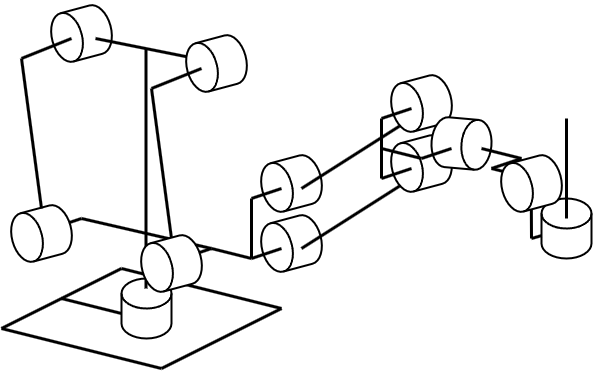
\includegraphics[width=70mm, keepaspectratio]{figures/Diagrammok/Diploma_kinematika}
\caption{Diploma munka kinematika}
\label{fig:Diploma_kinematika}
\end{figure}

A \ref{fig:Telemnanipulátor_kinematika}.ábrán láthatóan az elkészült telemanipulátor oldalról. A képen jól látható, hogy az meghatározott kinematikai lánc teljes egészében megvalósításra került. A megvalósításnál kifejezetten nagy kihívást jelentett az, hogy a karok vastagságát milyen méretűre válasszam meg. Kinematikai váz felrajzolásánál a geometriai elemek térbeli korlátjával érthető módon nem kellett foglalkozzak viszont megvalósításánál ez korlátozó tényező már nehézséget okozott.

\begin{figure}[!ht]
\centering
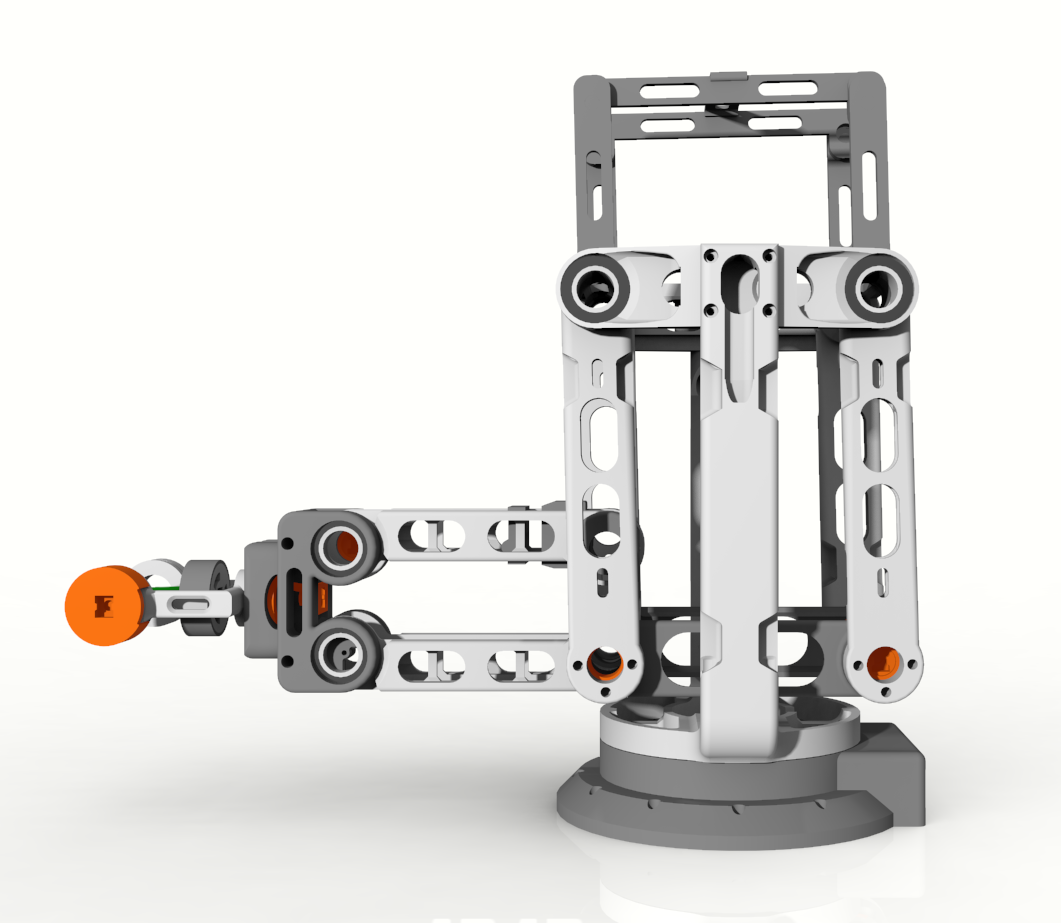
\includegraphics[width=120mm, keepaspectratio]{figures/Diploma_CAD/creo2.png}
\caption{Telemnanipulátor kinematikai elrendezésének bemutatása}
\label{fig:Telemnanipulátor_kinematika}
\end{figure}

A diploma dolgozatomban már korábban is említettem, de a továbbfejleszthetőséget nagyon fontosnak tartom. A karokat úgy terveztem meg, hogy a későbbiekben ne kelljen minden áron az egészet kicserélni, ha új koncepciós megvalósítást készítek. A következő \ref{fig:kar}.ábrán és a \ref{fig:Csuklo_egyedul}.ábrán a második és harmadik csukló közötti kar látható, illetve a kar két végén lecsatlakoztatható idom. Az idom illeszkedik a csapágyba illetve a kar keresztmetszetén található kábel csatornát fordítja be a tengely irányába.

\begin{figure}[!ht]
\centering
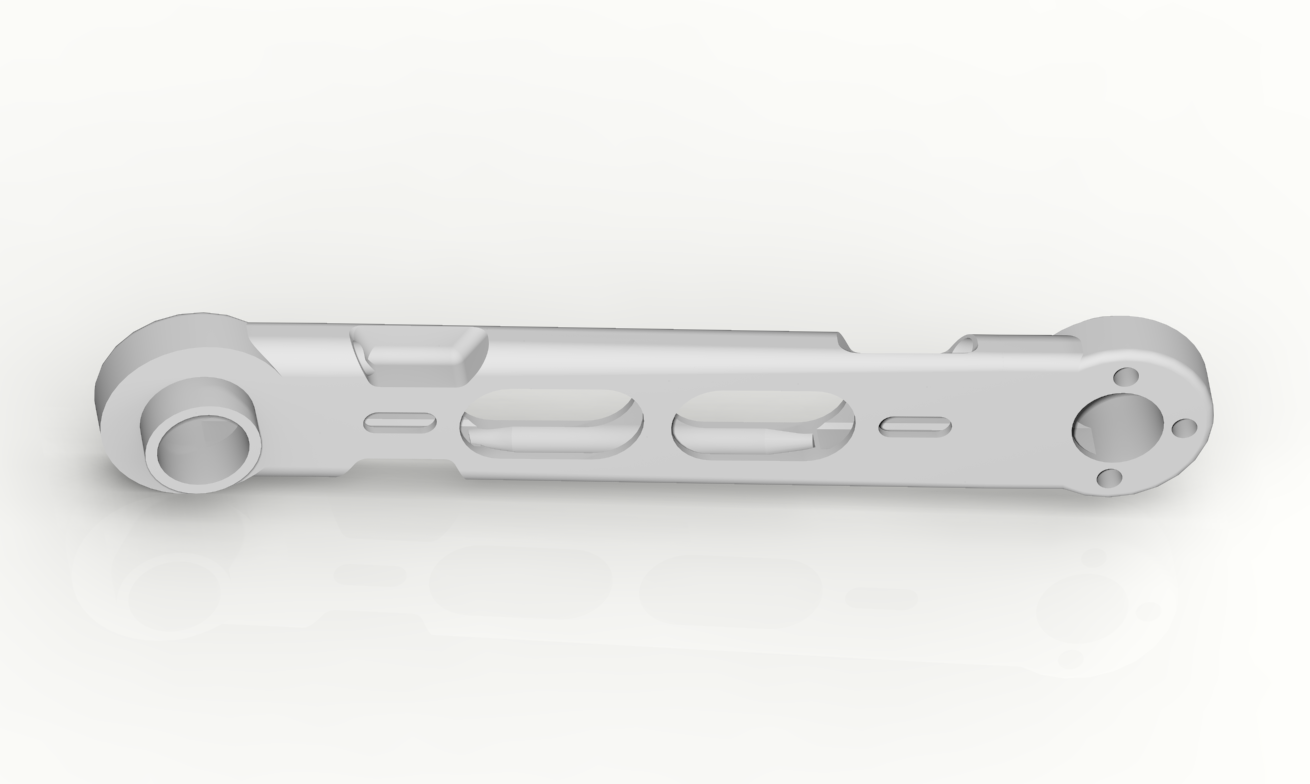
\includegraphics[width=150mm, keepaspectratio]{figures/Diploma_CAD/creo3.png}
\caption{Kar}
\label{fig:kar}
\end{figure}

Ez az idom csavarokkal van rögzítve a kar hosszanti testéhez. A karban réz inzerteket helyeztem így a csavart kellően feszesre meglehet húzni. A kar hosszanti elemén ovális kikönnyítéseket helyeztem el így kevesebb műanyagot használtam fel az elkészítésükhöz és könnyebbek lettek ezáltal, de a mechanikai tulajdonságaik megfelelnek az általam elvártaknak.

\begin{figure}[!ht]
\centering
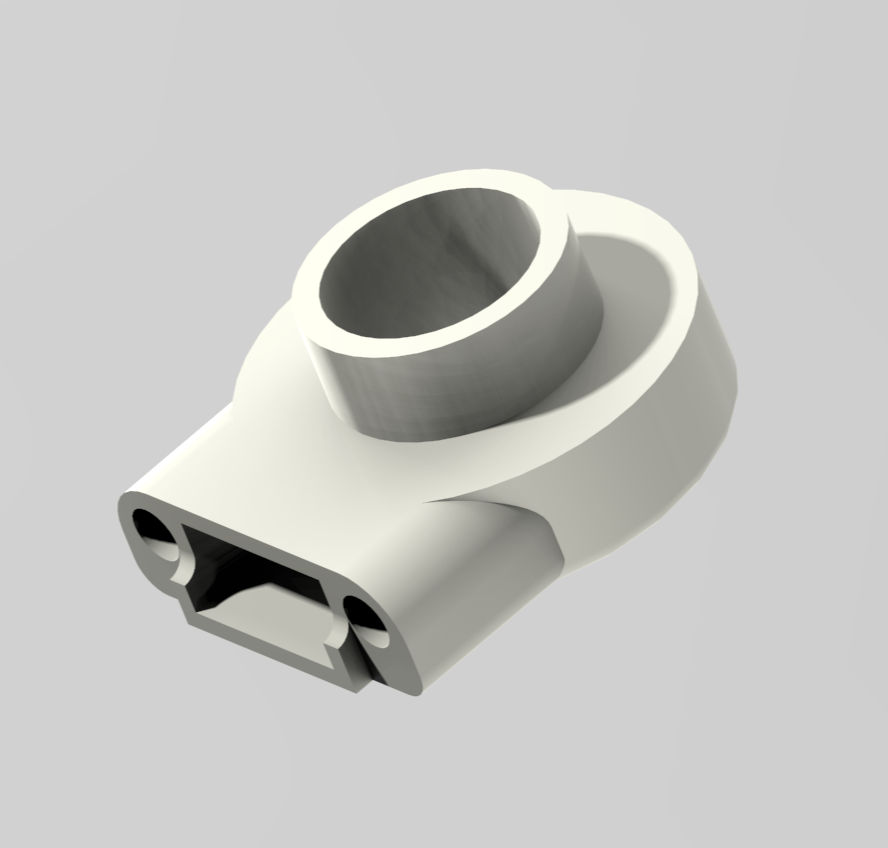
\includegraphics[width=70mm, keepaspectratio]{figures/Diploma_CAD/creo4.png}
\caption{Csuklo}
\label{fig:Csuklo_egyedul}
\end{figure}

A telemanipulátor minden egyes elemének bemutatását nem tartom fontosnak, mivel minden esetben a megfelelő mennyiségű kábel elvezethetőségét, a kellően nagy méretet és a optimális anyag felhasználást tartottam szem előtt. A következőképen a látható a teljes telemanipulátor. Az end-effektorról még ejtek párszót, de előtte a geometriai méreteket ismertetném és ezzel érzékelhetővé válik a szakdolgozatomban és az itt bemutatásra kerülő telemanipulátor méretbeli különbsége. A következő táblázat gyűjti össze a geometriai paramétereket.
\begin{table}[h!]
\centering
\begin{tabular}{ |c|c|c| }
 \hline
 Kar sorszám & Karhossza milliméterben  \\
 \hline
 Első kar & $290[mm]$  \\
 \hline
 Második kar & $200[mm]$  \\
 \hline
 Harmadik kar & $150[mm]$  \\
 \hline
 Negyedik kar & $87.5[mm]$  \\
 \hline
 Ötödik kar & $48[mm]$  \\
 \hline
 Hatodik kar & $30[mm]$  \\
\hline
\end{tabular}
\caption{Telemanipulátor karjainak méretét megadó táblázat}
\label{table:merettabla}
\end{table}

\begin{figure}[!ht]
\centering
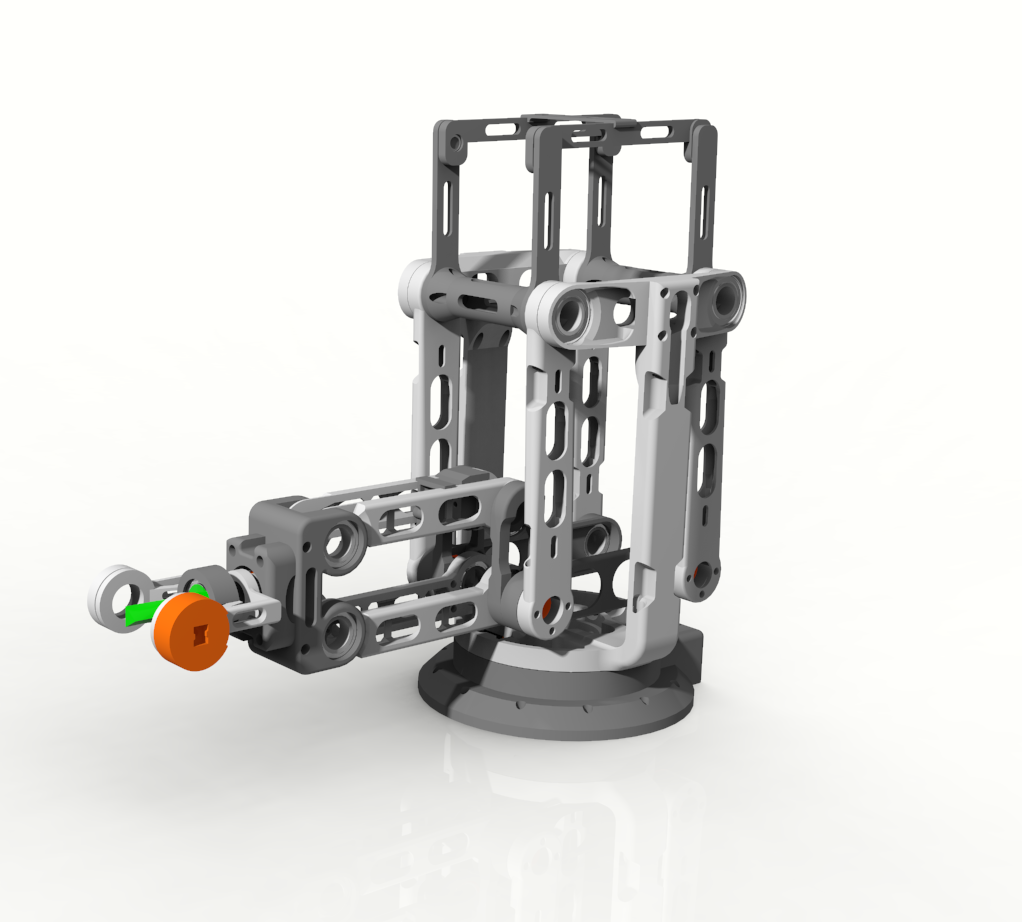
\includegraphics[width=120mm, keepaspectratio]{figures/Diploma_CAD/creo1.png}
\caption{Telemnanipulátor}
\label{fig:Telemnanipulátor}
\end{figure}

\section{Diplomamunkámban használt end-effektor}


\section{Kinematikai modell felépítése}

\begin{figure}[!ht]
\centering
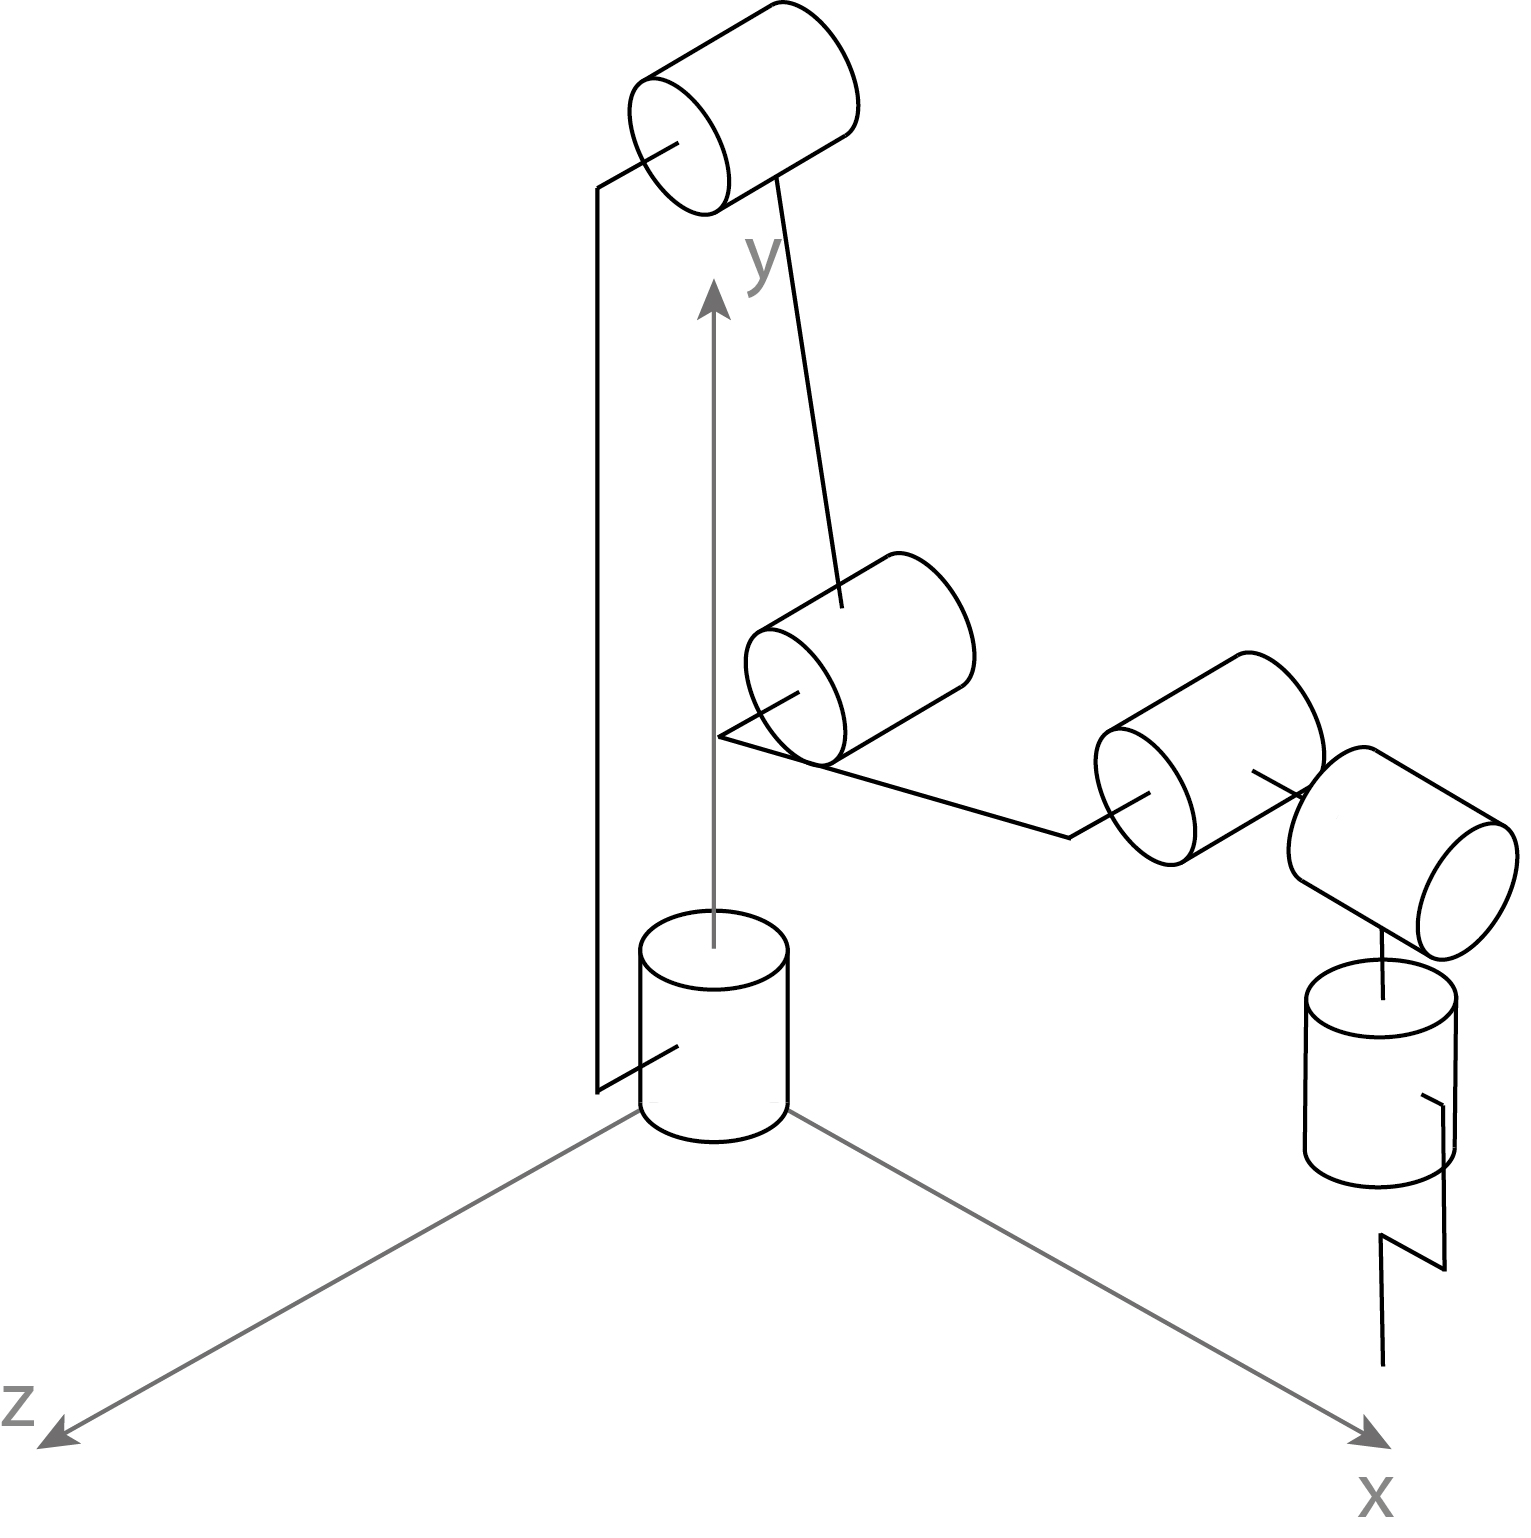
\includegraphics[width=70mm, keepaspectratio]{figures/Szakdoga/kinematik_v_2}
\caption{Szakdolgozat kinematika}
\label{fig:Csuklo_2}
\end{figure}

\begin{figure}[!ht]
\centering
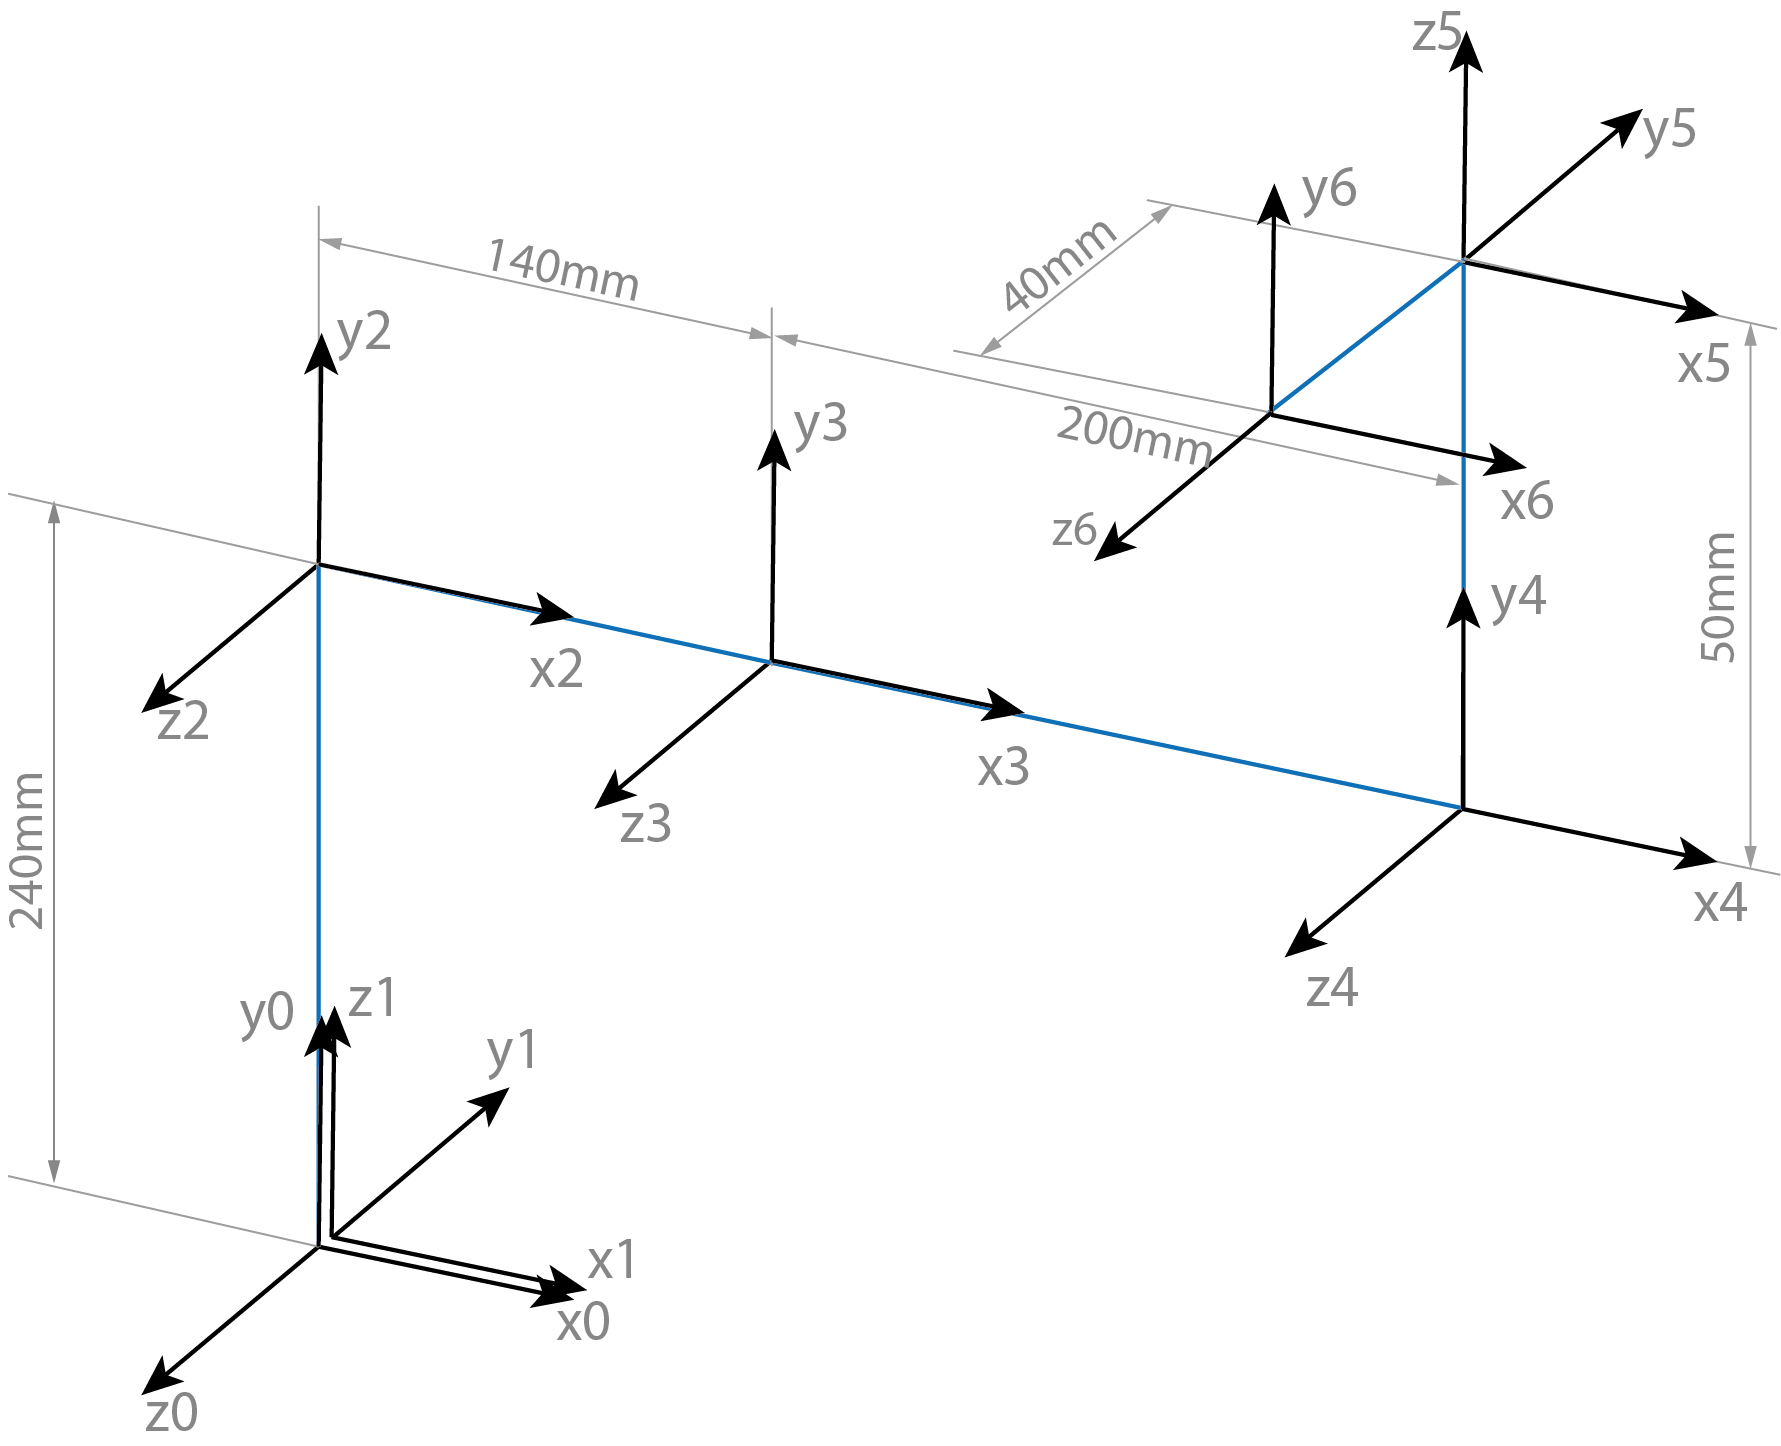
\includegraphics[width=70mm, keepaspectratio]{figures/Szakdoga/v_2_dh}
\caption{Szakdolgozat Denavit-Hartenberg felírás}
\label{fig:Csuklo_3}
\end{figure}


\begin{figure}[!ht]
\centering
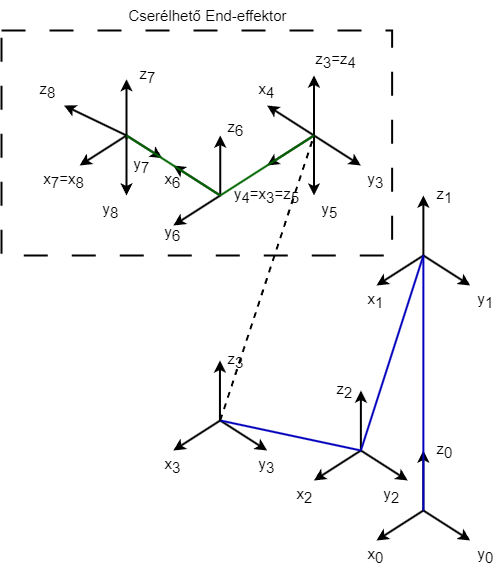
\includegraphics[width=70mm, keepaspectratio]{figures/Diagrammok/DH_feliras}
\caption{Diploma munka Denavit-Hartenberg felírás}
\label{fig:Csuklo_5}
\end{figure}



\subsection{Direkt kinematika}
%----------------------------------------------------------------------------
A direkt kinematika és a Khali-féle Denavit-Hartenberg (DH) módszer a robotika területén alkalmazott módszerek, amelyek lehetővé teszik a robotkarok és manipulátorok mozgásterének és pozíciójának meghatározását. Az alábbiakban bemutatom ezeket a módszereket és azok fő jellemzőit.

A direkt kinematika a robotkarok mozgásterének és végpontjainak pozíciójának meghatározását vizsgálja. Célja, hogy a robotkar ízületeinek állapotából vagy koordináta rendszeréből kiindulva meghatározza a végpont vagy a szerszám pozícióját a világkoordináta rendszerben. Ez a módszer matematikai modelleket és transzformációkat használ a kar szegmenseinek és ízületeinek geometriájának leírására és kapcsolatának meghatározására.

A Khali-féle DH módszer a direkt kinematika egyik legelterjedtebb módszere, amelyet a Denavit-Hartenberg (DH) paraméterek felhasználásával végeznek. Ez a módszer egy koordináta rendszer hierarchikus láncolását használja a robotkar szegmensei közötti kapcsolat leírására. A DH módszerben a kar szegmenseinek geometriáját és relatív helyzetét négy paraméter segítségével írják le: az alfa, a, d és theta paraméterek.

Az alfa paraméter az aktuális ízület tengelyének elfordulását jelenti a szomszédos szegmens tengelyéhez képest. Az a paraméter a szegmens hosszát vagy az ízület távolságát jelenti az előző szegmenstől. A d paraméter a szegmens központjának távolságát jelenti az előző szegmenstől a közös tengely mentén. A theta paraméter pedig az aktuális ízület elfordulását jelenti.

A DH módszerben minden szegmenst leíró paramétert és transzformációs mátrixot alkalmaznak, amelyek segítségével a végpont pozícióját határozzák meg. A módszer iteratív módon alkalmazható, a végponttól visszafelé haladva az egyes ízületek állapotának és pozíciójának meghatározására.

A direkt kinematika és a DH módszer széles körben alkalmazott eszközök a robotika területén. Segítségükkel lehetőség nyílik a robotkarok mozgásának tervezésére, szimulációjára és vezérlésére. Ezen módszerek alkalmazásával pontosan meghatározható a robotkar végpontjának helyzete és orientációja a világkoordináta rendszerben, ami fontos információ lehet a munkafolyamatok tervezésében és végrehajtásában.

Összességében a direkt kinematika és a Khali-féle DH módszer lehetővé teszik a robotkarok mozgásterének és pozíciójának meghatározását. Ezek a módszerek alapvetőek a robotika területén, és fontos szerepet játszanak a robotkarok tervezésében, szimulációjában és vezérlésében. A direkt kinematika és a DH módszer segítségével precízen modellezhetők és kontrollálhatók a robotkarok mozgásai, amelyek számos ipari és egyéb alkalmazásban hasznosak lehetnek.

\subsection{Inverz kinematika}
%----------------------------------------------------------------------------
Az inverz kinematika a robotika területén használt módszer, amely lehetővé teszi a robotkarok számára, hogy meghatározzák az ízületeik állapotát és pozícióját a kívánt végpont vagy TCP (tool center point) eléréséhez. Ez a módszer a direkt kinematika ellentéte, mivel itt nem a végpont pozícióját kell meghatározni az ízületek ismert állapota alapján, hanem éppen fordítva: az ízületek állapotát kell meghatározni a kívánt végpont pozíciója alapján.

Az inverz kinematika alkalmazása során a robotkar rendszerének geometriáját és ízületeinek korlátait figyelembe véve meg kell határozni az ízületek szögét vagy állapotát, amelyekkel a TCP a kívánt pozícióba kerül. Ez egy matematikai probléma, amelyet általában numerikus vagy analitikus megoldó algoritmusok segítségével oldanak meg.

Az inverz kinematika számos alkalmazási területtel rendelkezik a robotikában. Például a gyártósorokon, ahol a robotkaroknak pontosan kell pozícionálniuk a szerszámokat vagy alkatrészeket, az inverz kinematika segítségével a kívánt végpont pozíció alapján meg lehet határozni az ízületek állapotát. Ez lehetővé teszi a robotkarok pontos és ismételhető mozgását a gyártási feladatok hatékony végrehajtása érdekében.

A Khali-féle DH módszer a robotkarok leírására és az inverz kinematika alkalmazására is használt módszer. Ennek során a robotkar ízületeinek és szegmenseinek geometriáját és kapcsolatát a Denavit-Hartenberg (DH) paraméterek segítségével írják le. Ezek a paraméterek az alfa, a, d és theta értékekből állnak, amelyek meghatározzák az ízületek elfordulását és a szegmensek geometriáját.

A DH paraméterekkel leírt robotkar geometriáját felhasználva a Khali-féle DH módszerrel meghatározható az inverz kinematika. Az algoritmus segítségével a kívánt végpont vagy TCP pozíciója alapján a szükséges ízületi szög vagy állapot meghatározható. Az így kapott eredményeket a robotvezérlő egység továbbítja a robotkar motorjainak, hogy a megfelelő pozícióba mozgassa a TCP-t.

Az inverz kinematika és a Khali-féle DH módszer együttműködve lehetővé teszik a robotkarok számára, hogy a kívánt végpont vagy TCP pozíciókba helyezkedjenek el. Ez kulcsfontosságú a precíz munkavégzéshez és a különböző feladatok hatékony végrehajtásához a robotika számos alkalmazási területén, például az ipari automatizációban, a gyártásban, a logisztikában és a sebészeti beavatkozásokban. Az inverz kinematika és a Khali-féle DH módszer jelentős fejlődést hozott a robotkarok irányításában és pozícionálásában, és további lehetőségeket teremt a robotika területén.